% CS F407 Artificial Intelligence: final project report (course template, unmodified layout).
% Limit (updated 22 Nov 2026): 4 double-column pages including references.
\documentclass[11pt,a4paper,twocolumn]{article}

\usepackage[margin=2cm,columnsep=0.8cm]{geometry}
\usepackage[T1]{fontenc}
\usepackage{lmodern}
\usepackage{microtype}
\usepackage{amsmath,amssymb}
\usepackage{graphicx}
\usepackage{booktabs}
\usepackage{tabularx}
\usepackage{enumitem}
\usepackage{titlesec}
\usepackage[hidelinks]{hyperref}

\titleformat{\section}{\normalsize\bfseries}{\thesection}{0.6em}{}
\titlespacing*{\section}{0pt}{1.2ex plus 0.3ex}{0.6ex}
\setlist{nosep,leftmargin=*}
\setlength{\parskip}{0.3ex}

\newcommand{\coursename}{CS F407 Artificial Intelligence, AY 2026--27 Semester I}
\newcommand{\teamno}{Team Artificially Intelligent}
\newcommand{\githuburl}{https://github.com/RaghavSinghal15/indus-computational-epigraphy}

\newcommand{\AGRIMID}{2024XXXXXXXG}
\newcommand{\DETECTORTEXT}{}
\begin{document}

\twocolumn[{%
\begin{center}
  {\large\bfseries Measuring the Structure of the Undeciphered Indus Script:\\ Seal Reading, Sign Statistics and Guardrails}\\[1ex]
  \teamno\\
  Raghav Singhal (2024ADPS0827G), Devam Jatin Bhavsar (2024ADPS0831G), Krrish Bagaria (2024A7PS0507G),\\ Saatwik Tiwari (2024ADPS0878G), Agrim Agarwal (\AGRIMID)\\[0.5ex]
  {\small \coursename, BITS Pilani, K.K. Birla Goa Campus}\\[1.5ex]
  \begin{minipage}{0.85\textwidth}
    \small
    \centerline{\bfseries Abstract}\vspace{0.5ex}
    The Indus script survives on about 4,000 short inscriptions and is undeciphered. We do not try to read it; we measure its structure and test how far each measurement can be trusted. We built 855 labelled seal photographs with 4,078 hand-checked sign boxes, and a reader that turns a photo into Wells sign IDs: 33.7\% first-guess accuracy on unseen seals with forced cuts, 73.9\% when the CNN is trained and tested on hand-box crops, and similar accuracy on a site never trained on. Synthetic inscriptions built from real sign crops (suggested by Prof.\ Ashwin) lower a whole-band CRNN's sign error on that unseen site from 57.9\% to 53.2\%. On the sign sequences, Markov statistics, masked prediction (35\% top-1) and Naive Bayes guardrails (81\% real vs shuffled) show strong order, but non-linguistic symbols pass the same test and a no-language Markov chain reproduces most classic statistics; only sign triples set the script apart.
  \end{minipage}
\end{center}
\vspace{1.5ex}
}]

\section{Introduction}
The Indus script (c.\ 2600--1900 BCE) is known from short texts, mostly on seals, averaging under five signs. Decipherment claims are frequent and unverifiable, so we ask a narrower question: what can standard AI methods measure about the script's structure, and how reliable is each measurement? \textbf{Input:} a seal photograph, or a sign sequence from a corpus. \textbf{Output:} the ordered sign IDs, statistics of sign order, predictions of hidden signs, and tests against null models.

\textbf{Contributions.} (i) A labelled set of 855 seal photos with 4,078 hand-checked sign boxes on a fixed seal-level split; (ii) a seal reader (M1) evaluated on unseen seals and an unseen site; (iii) synthetic inscriptions composed from real sign crops; (iv) Markov statistics (M2), masked prediction (M3) and guardrails (M4), with two extensions: how M1's errors distort M2--M4 (E1) and what a no-language process can already reproduce (E2).

\section{Background and related work}
Statistical work on the script uses Mahadevan's concordance~\cite{mahadevan1977} and the ICIT corpus with Wells sign numbers~\cite{fuls2022}. Rao et al.~\cite{rao2009} argued from conditional entropy that the script is linguistic; Yadav et al.~\cite{yadav2010plos} fitted $n$-gram models (bigram perplexity 26.7) and restored doubtful signs. Sproat~\cite{sproat2014} showed that non-linguistic symbol systems can pass such tests. On the vision side, Dixit et al.~\cite{dixit2025} report 94.5\% on about 40 common signs with crop-level splits. We use standard tools: CNNs, HMM forward--backward decoding, CRNNs with CTC loss~\cite{graves2006ctc}, synthetic training text in the spirit of SynthText~\cite{gupta2016synthtext}, smoothed $n$-grams, transformers and Naive Bayes.

\section{Method}
\textbf{Data.} Sequences use Wells IDs. The M2--M4 benchmark is the 1,837-text corpus of~\cite{yadav2010plos} (8,359 signs, 568 types). Seal photos are CISI scans~\cite{cisi1}; we first linked 328 to the concordance by hand, then took sequences for 855 seals from Lipi~\cite{lipi}, a digitised copy of Fuls's corpus (96.5\% agreement with our labels). M1 predicts Wells IDs (712 classes), so its output feeds M2--M4 without cross-scheme mapping. The team drew a tight box around every sign on 834 seals in a browser tool; labels come automatically from the known sequence and a checker rejects any seal whose box count is wrong.

\textbf{M1, cut and classify.} Find the text band from the row profile of a carving mask; cut it into $n$ pieces, moving each cut to the lowest-ink column within $\pm$30\% of an equal split; classify each $64{\times}64$ crop with a 4-block CNN (Conv--BN--ReLU, global average pooling, dropout, softmax), pretrained on 35,600 carved-look renders of clean sign drawings and fine-tuned on real crops; decode with an HMM whose emissions are CNN probabilities and transitions ICIT sign-pair probabilities (forward--backward, weight chosen on validation).

\textbf{M1, reading without cutting.} A CRNN uses the CNN as a column-feature extractor, a BiLSTM over columns in reading order, and CTC loss, so it needs neither a sign count nor boxes.

\textbf{Compositor.} Following Prof.\ Ashwin's suggestion, we generate inscriptions from real signs: hand-boxed crops of training seals are pasted, in the order of real ICIT texts, onto real seal surfaces whose signs were removed by inpainting, with brightness matching, feathered edges, random spacing and photo noise. Only training seals and texts absent from held-out seals are used (2,240 crops of 336 signs, 1,260 texts, 5,000 composites, each with its sequence and boxes).

\textbf{M2--M3.} Sign and pair frequencies with start/end markers; empirical next-sign entropy in each direction. For masked prediction we score each candidate $s$ between neighbours $L,R$ by $P(s\mid L)\,P(R\mid s)$ with Witten--Bell smoothed bigrams, $P(b\mid a)=\frac{c(a,b)+T(a)P_{\text{uni}}(b)}{c(a)+T(a)}$, where $T(a)$ counts distinct successors of $a$. A small masked transformer is the neural comparison.

\textbf{M4 and extensions.} Naive Bayes over bags of adjacent pairs separates real texts from within-text shuffles; single signs (unchanged by shuffling) are the control; 1,000-shuffle permutation tests check entropy and jar-final rates. E1 corrupts the corpus to a given reading accuracy, by random or by the CNN's measured confusions, and reruns M2--M4. E2 fits unigram and bigram generators to the corpus and asks which statistics they reproduce. Both are also run on Sproat's non-linguistic corpora~\cite{sproat2014}.

\section{Experimental setup}
One fixed seal-level split: 466 train, 67 validation, 141 test seals (first-phase test and validation seals keep their roles), and all 181 Harappa seals held out for a cross-site test. Text experiments use a fixed 1,469/368 split. Every choice was made on validation; test numbers are reported once. Metrics: top-1/top-5 sign accuracy; sign error rate (SER: insertions, deletions and substitutions over reference signs); perplexity; held-out classifier accuracy. Hardware: Colab T4 GPU and a 2-core CPU; PyTorch, OpenCV, Ultralytics; seed 0 throughout.

\begin{table}[t]
\centering\small\setlength{\tabcolsep}{4pt}
\begin{tabular}{@{}lr@{}}
\toprule
Reader (sign count given) & Top-1 / Top-5 \\
\midrule
Most frequent signs & 11.4 / 24.9 \\
v1 CNN, Mahadevan IDs (matched) & 29.7 / 48.0 \\
v2 CNN, Wells IDs (matched) & 35.5 / 58.4 \\
\midrule
v2 CNN, forced cuts & 31.0 / 52.3 \\
v2 CNN + ICIT bigram, forced cuts & 33.7 / 55.1 \\
v2 CNN, hand-box crops & 52.8 / 77.7 \\
Hand-box-trained CNN, hand boxes & \textbf{73.9} / \textbf{90.1} \\
\midrule
Harappa, v2 CNN, cuts & 28.9 / 48.8 \\
Harappa, hand-box-trained CNN & 71.3 / 91.2 \\
\bottomrule
\end{tabular}
\caption{M1 sign accuracy (\%, higher is better) on 141 test seals (686 signs) unless stated. Matched rows: the 279 positions shared by v1 and v2. Harappa: 181 seals never used in training.}
\label{tab:m1}
\end{table}

\begin{figure*}[t]
\centering
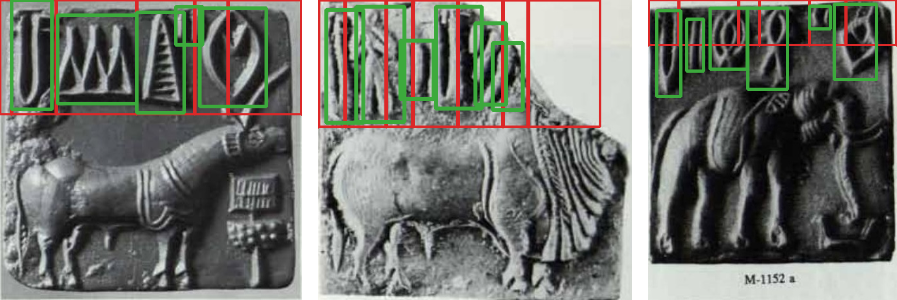
\includegraphics[height=3.2cm]{figures/segmentation_cuts_vs_boxes.png}\hfill
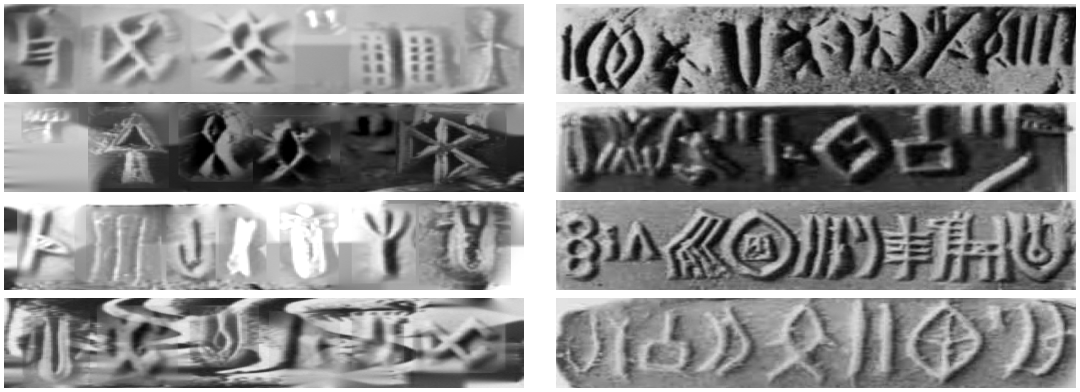
\includegraphics[height=3.2cm]{figures/composites_vs_real.png}
\caption{Left: forced cuts (red, true count given) vs reviewed hand boxes (green) on test seals; cuts slice signs. Right: composites built from real sign crops along real texts (left column) next to real training bands.}
\label{fig:m1}
\end{figure*}

\section{Results}
\textbf{M1.} Table~\ref{tab:m1}. On the same test signs v2 beats v1 by 6 points. Accuracy follows sign frequency: 44.6\% for signs with 20+ training crops, 4.3\% for signs never seen in real training. The reader transfers across sites: a model trained on Mohenjo-daro gets 29.9\% there and 28.9\% on Harappa. Collapsing our task to Dixit et al.'s 40-sign label set raises top-1 from 35.0\% to 62.5\% (majority baseline 49.9\%), and a random crop split did not raise it further, so most of the gap to 94.5\% is the task, not the model.

\textbf{Segmentation is the bottleneck.} On 64 test seals forced cuts reach mean IoU 0.455 with the hand boxes and isolate only 21 of 322 signs cleanly (Fig.~\ref{fig:m1}); the same CNN reads 33.2\% of these signs from our cuts and 55.9\% from hand-box crops. Training on hand-box crops instead of cuts (same start, same extra epochs) lifts hand-box test accuracy from 55.7\% to 73.9\%, but the model drops to 28.6\% on forced cuts, so the gain needs good boxes at test time. \DETECTORTEXT

\begin{table}[t]
\centering\small\setlength{\tabcolsep}{4pt}
\begin{tabular}{@{}lrrr@{}}
\toprule
Reader & SER & Exact & Count \\
\midrule
Cut + CNN, count given & 68.1 & 2.1 & 100 \\
Cut + CNN, count estimated & 113.8 & 1.4 & 16.3 \\
CRNN, real bands & 55.4 & 4.3 & 27.7 \\
CRNN, real + composites & \textbf{54.4} & 3.5 & \textbf{29.1} \\
\midrule
\multicolumn{4}{@{}l}{\emph{Harappa (181 seals, never trained on)}}\\
CRNN, real bands & 57.9 & 5.5 & 29.3 \\
CRNN, real + composites & \textbf{53.2} & \textbf{7.7} & \textbf{35.9} \\
\bottomrule
\end{tabular}
\caption{Whole-inscription reading on 141 test seals: sign error rate (lower is better), exact inscriptions and correct sign count (\%). CRNN rows share seed and settings.}
\label{tab:crnn}
\end{table}

\textbf{Reading without cutting; composites.} The CRNN needs no count and beats cut-and-classify even when that is given the count (Table~\ref{tab:crnn}). Adding the 5,000 composites lowers test SER only slightly (within single-seed noise), but on Harappa SER falls by 4.7 points and correct counts rise from 53 to 65 of 181 seals: composites add arrangements and backgrounds that the 466 real bands lack, which matters most when test photos differ from training ones.

\textbf{M2.} 568 sign types follow a Zipf-like curve (top 10 signs: 33\% of tokens; 39\% of types occur once). The jar sign (Wells 740) ends 35.2\% of texts and begins 0.16\%. Next-sign entropy is 3.31 bits in reading order and 3.82 reversed. On the full ICIT corpus every statistic moves by under a point; by site, the jar sign ends 39.6\% of Mohenjo-daro texts but 29.0\% of Harappa texts.

\textbf{M3.} Masked top-1/top-5: unigram 11.3/23.7\%, previous sign only 25.0/44.9\%, both neighbours 35.0/60.0\%. Held-out perplexity is 87.1 (unigram) and 37.8 (bigram), close to the published 68.8 and 26.7 on a different corpus~\cite{yadav2010plos}. The best of four transformer variants over three seeds reached 29.9/52.0\%, below a trigram (35.8/61.0\%).

\begin{figure}[t]
\centering
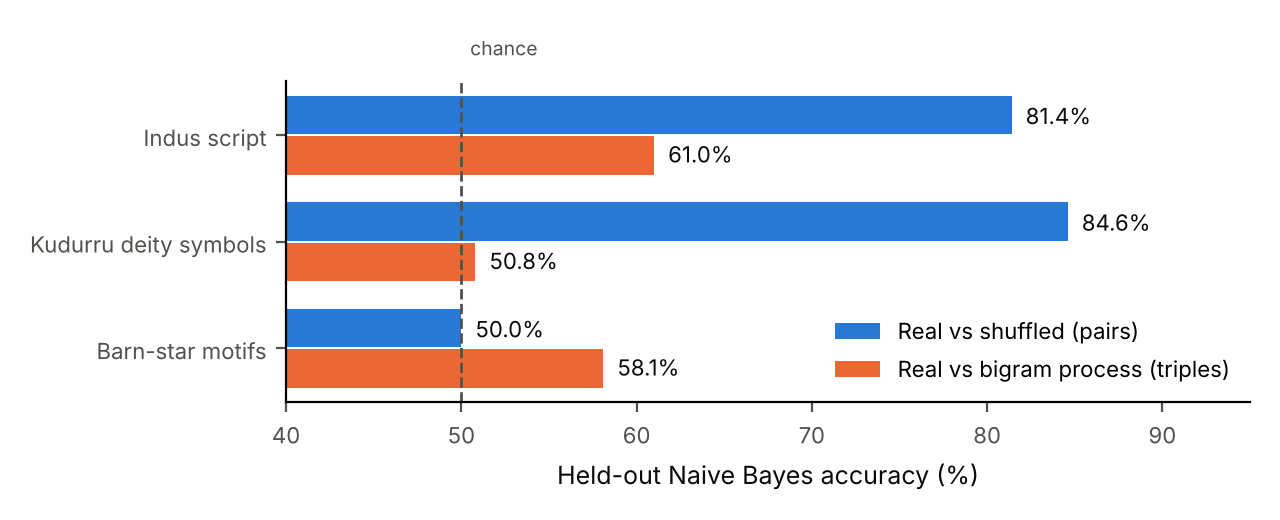
\includegraphics[width=\linewidth]{figures/guardrails_controls.png}
\caption{Order tests on the Indus corpus and two non-linguistic systems. Blue: real vs shuffled (pairs). Orange: real vs a fitted bigram process (triples). Dashed: chance.}
\label{fig:guard}
\end{figure}

\textbf{M4.} Naive Bayes separates real from shuffled texts with 81.4\% accuracy (control 50.0\%); permutation tests give entropy 3.685 vs 4.715 bits and jar-final 35.2\% vs 11.1\% ($p=0.001$ for both). But Mesopotamian kudurru deity symbols, which are not writing, also pass (84.6\%), while barn-star motifs do not (50.0\%) (Fig.~\ref{fig:guard}): non-random order alone is not evidence of language.

\textbf{E1.} Real-vs-shuffled accuracy falls from 82.7\% with perfect readings to 64.5\% at 60\% reading accuracy and 53.5\% at 30\%; the jar sign's final position survives longer ($p=0.005$ at 30\%). With the CNN's measured confusions at the same 31\% accuracy more structure survives (61.0\% vs 53.8\%), because a reader confuses similar signs consistently.

\textbf{E2.} A bigram chain with no words or grammar reproduces Zipf's slope ($-0.93$), the jar-final rate (37.6\% vs 35.2\%) and similar entropy (3.00 vs 3.31 bits). Pairs cannot tell its output from real texts (49.6\%), but triples can (61.0\%, control 49.0\%); deity symbols show no such excess (50.8\%).

\section{Discussion and limitations}
The reader's limit is segmentation, not recognition: with good boxes the CNN reaches 74\%, so a trained detector, or a CRNN trained on many more composites, is the next step. Statistics computed from automatic readings at today's accuracy would mostly describe the reader (E1). Each experiment uses one seed and one split; test sets of 141 and 181 seals give roughly $\pm$4 points. Most of the 712 sign classes have few or no real examples. Boxes for batches 7--9 (mostly Harappa) were AI-assisted and then checked, and are less reliable than batches 1--6. Small control corpora are noisy: barn stars give 58.1\% on triples while their own control gives 45.7\%.

\section{Conclusion}
Sign order in the Indus texts is strongly structured and partly predictable, and real sign crops recombined along real texts make a useful training resource. But order alone does not separate the script from non-linguistic symbols or from a simple Markov process; recurring sign groups beyond pairs are the property here that does.

\section*{Individual member contributions}
{\small
\begin{tabularx}{\linewidth}{@{}l X@{}}
\toprule
Name & Contribution \\
\midrule
Raghav Singhal & Lead; plan and repository; M1 v1 (segmentation, CNN, renders, decoder, count search); Lipi import, Wells switch, fixed split; box protocol and tools; compositor, composite and hand-box experiments; M3, M4, E1, E2 baselines; boxes for batches 7--9; integration, report, video. \\
Devam J. Bhavsar & M2 statistics; v2 CNN training and v1/v2 comparison; CRNN; segmentation audit; Harappa, Dixit-protocol and CNN-confusion studies; neural M3; full-corpus and non-linguistic controls; detector pipeline; boxes for batches 1 and 6. \\
Krrish Bagaria & Found the CISI-to-concordance link; first labelled seal set (with Saatwik); reviewed boxes for batches 2 and 5; flash-talk slides. \\
Saatwik Tiwari & First labelled seal set (with Krrish); literature review; reviewed boxes for batch 3. \\
Agrim Agarwal & First synthetic sign generator; first-pass boxes for batches 2--6; reviewed boxes for batch 4. \\
\bottomrule
\end{tabularx}}

\smallskip
\noindent All members have read this report and agree with the statement above.

\section*{Generative AI disclosure}
We used Claude (Anthropic; Claude Code and claude.ai) and ChatGPT/Codex (OpenAI) to discuss approaches, write, review and debug code under our supervision, draft documentation, edit this report, and pre-draw sign boxes for batches 7--9, which we then checked. In the first phase ChatGPT transcribed 47 seals we could not verify by hand; they were marked and used only for training. No generative model is part of the method itself. We checked all such output, every number here is produced by code in the repository and checked against a known value, and we take responsibility for it.

\section*{Code availability}
\noindent Code and data:\\
\url{\githuburl}\\
The README lists every result with the report and command that reproduces it.

\begin{thebibliography}{9}
\small
\bibitem{cisi1} J.~P.~Joshi and A.~Parpola (eds.). \emph{Corpus of Indus Seals and Inscriptions, Vol.~1}. Suomalainen Tiedeakatemia, 1987.
\bibitem{dixit2025} Dixit, Hussain, Basak, Atturu, D.~Mitra and U.~Bhattacharya. Deep learning in archiving Indus script and motif information. \emph{J. Computer Applications in Archaeology}, 2025.
\bibitem{fuls2022} A.~Fuls. \emph{Corpus of Indus Inscriptions}. Harrassowitz, 2022.
\bibitem{graves2006ctc} A.~Graves, S.~Fern\'andez, F.~Gomez and J.~Schmidhuber. Connectionist temporal classification. \emph{ICML}, 2006.
\bibitem{gupta2016synthtext} A.~Gupta, A.~Vedaldi and A.~Zisserman. Synthetic data for text localisation in natural images. \emph{CVPR}, 2016.
\bibitem{lipi} Yajnadevam. Lipi: Indus inscriptions and seal images. \url{https://github.com/yajnadevam/lipi}, commit fc8813a (metadata and photos only).
\bibitem{mahadevan1977} I.~Mahadevan. \emph{The Indus Script: Texts, Concordance and Tables}. Archaeological Survey of India, 1977.
\bibitem{rao2009} R.~P.~N.~Rao et al. Entropic evidence for linguistic structure in the Indus script. \emph{Science} 324:1165, 2009.
\bibitem{sproat2014} R.~Sproat. A statistical comparison of written language and nonlinguistic symbol systems. \emph{Language} 90(2):457--481, 2014.
\bibitem{yadav2010plos} N.~Yadav et al. Statistical analysis of the Indus script using $n$-grams. \emph{PLoS ONE} 5(3):e9506, 2010.
\end{thebibliography}

\end{document}
